%%%%% Single page layout:
%%%%% ----------------------------------------------------
%\documentclass[12pt, a4paper,draft]{report}
\documentclass[12pt, a4paper]{report}
\setlength\textwidth{160mm}
\setlength\textheight{247mm}
\setlength\oddsidemargin{0mm}
\setlength\evensidemargin{0mm}
\setlength\topmargin{0mm}
\setlength\headsep{0mm}
\setlength\headheight{0mm}
\let\openright=\clearpage
% Overfull statements
\pretolerance=150
\setlength{\emergencystretch}{3em}
% Overfull end

\usepackage[utf8]{inputenc}


%%% Additional useful packages
%%% ----------------------------------------------------------------
\usepackage{array}
\usepackage{amsmath}  
\usepackage{amssymb}
\usepackage{amsfonts}
\DeclareFontFamily{OT1}{pzc}{}
\DeclareFontShape{OT1}{pzc}{m}{it}{<-> s * [0.900] pzcmi7t}{}
\DeclareMathAlphabet{\mathpzc}{OT1}{pzc}{m}{it}
\usepackage{amsthm}      
\usepackage[ruled,algochapter]{algorithm2e}
\usepackage{algorithmic}
\usepackage{bm}
\usepackage[mathscr]{euscript}
\usepackage{graphicx}       
\usepackage{psfrag}         
\usepackage{fancyvrb}    
\usepackage{float}
\usepackage{ltablex}
\usepackage[square,sort,comma,numbers]{natbib}        
\usepackage{bbding}         
\usepackage{dcolumn}        
\usepackage{booktabs} 
\usepackage{multirow}
\usepackage{paralist}       
\usepackage{indentfirst}    
\usepackage[nottoc,notlof,notlot]{tocbibind}
\usepackage{url}
\usepackage{tabularx}
\usepackage{subcaption}
\usepackage[unicode]{hyperref}
\usepackage{xcolor}

\hypersetup{pdftitle=LiDAR obstacle detection and avoidance, 
            pdfauthor=Alojz Gomola,
            colorlinks=false,
            urlcolor=blue,
            pdfstartview=FitH,
            pdfpagemode=UseOutlines,
            pdfnewwindow,
            breaklinks
          }
\usepackage{array}
\newcolumntype{L}[1]{>{\raggedright\let\newline\\\arraybackslash\hspace{0pt}}m{#1}}
\newcolumntype{C}[1]{>{\centering\let\newline\\\arraybackslash\hspace{0pt}}m{#1}}
\newcolumntype{R}[1]{>{\raggedleft\let\newline\\\arraybackslash\hspace{0pt}}m{#1}}         
\newcolumntype{B}{X}
\newcolumntype{S}[1]{>{\hsize=#1\textwidth}X}

\newcommand{\FIGDIR}{./Pics}    %%% directory containing figures
\newcommand{\twolinecellr}[2][r]{%
  \begin{tabular}[#1]{@{}r@{}}#2\end{tabular}}
\theoremstyle{plain}
\newtheorem{theorem}{Theorem}
\newtheorem{lemma}[theorem]{Lemma}
\newtheorem{proposition}[theorem]{Proposition}

\theoremstyle{plain}
\newtheorem{definition}{Definition}
\newtheorem{problem}{Problem}
\newtheorem{example}{Example}
\newtheorem{assumption}{Assumption}

\theoremstyle{remark}
\newtheorem*{corollary}{Corollary}
\newtheorem*{note}{Note}




\newenvironment{dokaz}{
  \par\medskip\noindent
  \textit{Proof}.
}{
\newline
\rightline{\SquareCastShadowBottomRight}
}

\newenvironment{constraints}[1]{
  \par\medskip\noindent
  \textit{Constraints #1} \\
}{
\newline
\rightline{\SquareCastShadowBottomRight}
}


%\bibliographystyle{plainnat}     %% Author (year) style
\bibliographystyle{unsrt}        %% [number] style
\setcitestyle{square}

% Section  3.7 Challenge list
\newif\ifproblemchallenge   %# Build block for problem challenges
\problemchallengetrue       %# Show comments


\title{Dissertation thesis}
\author{Alojz Gomola}
\date{February 2019}

%%%%% ------------------------------------------------------------
\DefineVerbatimEnvironment{PCinout}{Verbatim}{fontsize=\small, frame=single}



\newcommand{\R}{\mathbb{R}}
\newcommand{\N}{\mathbb{N}}

\DeclareMathOperator{\pr}{\textsf{P}}
\DeclareMathOperator{\E}{\textsf{E}\,}
\DeclareMathOperator{\var}{\textrm{var}}
\DeclareMathOperator{\sd}{\textrm{sd}}


\newcommand{\T}[1]{#1^\top}        

\newcommand{\goto}{\rightarrow}
\newcommand{\gotop}{\stackrel{P}{\longrightarrow}}
\newcommand{\maon}[1]{o(n^{#1})}
\newcommand{\abs}[1]{\left|{#1}\right|}
\newcommand{\dint}{\int_0^\tau\!\!\int_0^\tau}
\newcommand{\isqr}[1]{\frac{1}{\sqrt{#1}}}
\newcommand{\norm}[1]{\left\lVert#1\right\rVert}


\newcommand{\pulrad}[1]{\raisebox{1.5ex}[0pt]{#1}}
\newcommand{\mc}[1]{\multicolumn{1}{c}{#1}}
\newcommand{\TBD}[1]{\color{red}\emph{--TBD:}#1\color{black}}

\begin{document}

\setcounter{chapter}{6}
\setcounter{section}{4}

		
	%06-05 Moving Obstacles and Intruders	
    \subsection{Intruders}\label{s:intruders}
\paragraph{Intruder behavior:} \emph{Adversarial behavior} of moving obstacle is trying to destroy avoiding our UAS.  The \emph{Intruder} UAS \cite{fiorini1998motion} is not trying to hurt our \emph{UAS} actively. The \emph{Adversarial behaviour} is neglected in this work. The non-cooperative avoidance is assumed, it can be relaxed to \emph{cooperative avoidance} in \emph{UTM controlled airspace}.

\paragraph{Intruder information:} The \emph{observable intruder information set} for any kind of intruder, obtained through the sensor/C2 line, is following:
\begin{enumerate}
    \item\emph{Position} - position of an intruder in the \emph{local} or \emph{global} coordinate frame, which can be transformed into \emph{avoidance grid coordinate frame}.
    
    \item\emph{Heading and Velocity} - intruder heading and linear velocity in avoidance grid coordinate frame.
    
    \item\emph{Horizontal/Vertical Maneuver Uncertainty Spreads} - how much can an \emph{intruder} deviate from the \emph{original linear path} in a \emph{horizontal/vertical} plane in \emph{Global coordinate Frame}.
\end{enumerate}

 

\begin{figure}[H]
    \centering
    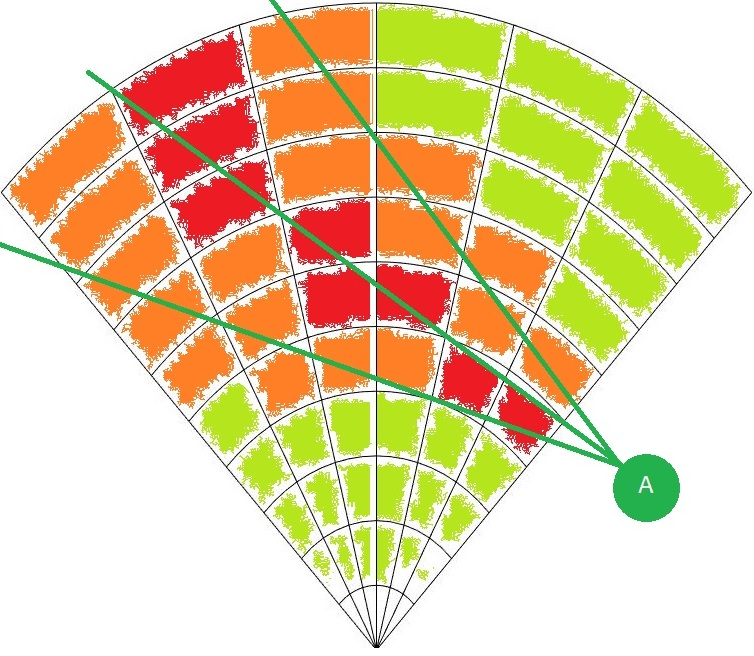
\includegraphics[width=0.7\textwidth]{\FIGDIR/TE052AdversaryProbabilitySpread}
    \caption{Intruder UAS intersection rate along the expected trajectory.}
    \label{fig:intruderProbabiltySpreadTheoretical}
\end{figure}   

\paragraph{Example of Intruder Intersection:} Let us neglect the \emph{time-impact} aspect on the \emph{intersection}.  The \emph{intruder} (black "I" circle) is intersecting one \emph{avoidance grid horizontal slice} (fig. \ref{fig:intruderProbabiltySpreadTheoretical}).  The intruder is moving along linear path approximation based on velocity (middle green line). The \emph{Horizontal Maneuver Uncertainty spread} is in \emph{green line boundary area} \emph{intruder intersection rating} is denoted as green-orange-red cell fill reflecting intersection severity:  red is a high rate of the intersection, orange is the medium rate of the intersection and green is a low rate of the intersection.
    


\paragraph{Moving Threats:} The \emph{UAS} can encounter following threats during the \emph{mission execution}:
\begin{enumerate}
    \item \emph{Non-cooperative Intruders} - the intruders who does not implement any approach to ensure mutual avoidance efficiency.
    
    \item \emph{Cooperative Intruders} - the intruders whom actively communicate or follow common agreed behavior pattern (ex. Rules of the Air).
    
    \item \emph{Moving Constraints} - the constrained portion of \emph{free} space which is shifting its boundary over time (ex. Short term bad weather).
\end{enumerate}
    
\begin{note}
    Our approach considers only \emph{UAS} intruders because \emph{Data Fusion} considers data received through \emph{ADS-B} messages. The \emph{Intruders} extracted from \emph{LiDAR} scan were not considered (ex. birds). The proposed \emph{intruder intersection models} are reusable for other \emph{intruder sources}.
\end{note}

\paragraph{Approach Overview:} The \emph{Avoidance Grid} (def. \ref{def:AvoidanceGrid}) is adapted to the \emph{LiDAR} sensor. The \emph{Euclidean grid intersections} are fairly simple. The \emph{polar coordinates grid} is not. The need to keep \emph{polar coordinates grid} is prevalent, because of fast \emph{LiDAR} reading assessment.  There are following commonly known methods to address this issue:

\begin{enumerate}
    \item\emph{Point-cloud Intersections} - the \emph{threat impact area} is discredited into a sufficiently thick point cloud. This point-cloud have \emph{point impact rate} and \emph{intersection time} assigned to each point. The \emph{point-cloud} is projected to \emph{Avoidance Grid}. If the \emph{impact point} hits $cell_{i,j,k}$ the cell`s impact rate is increased by the amount of \emph{point impact rate}. The final \emph{threat impact rate} in $cell_{i,j,k}$ is given when \emph{all} points from point cloud are consumed. Close point problem \cite{shamos1975closest} was solved by the application of method  \cite{bentley1980optimal}.
    
    \item\emph{Polygon Intersections} - the \emph{threat impact area} is modeled as a polygon, each $cell_{i,j,k}$ in \emph{Avoidance Grid} is considered as a \emph{polygon}. There is a possibility to calculate cell space geometrical inclusive intersection. The \emph{impact rate} is then given as rate between \emph{intersection volume} and $cell_{i,j,k}$ volume. The algorithm used for intersection selected based on:\citep{bentley1979algorithms} the selected algorithm  \emph{Shamos-Hoey} \cite{shamos1976geometric}.
\end{enumerate}

\begin{note}
    The \emph{Intruder Intersection} models are based on \emph{analytical geometry} for \emph{cones and ellipsoids} taken from \cite{sommerville2016analytical}.
\end{note}

    	\subsection{(R) Intruder Behaviour Prediction}\label{s:intruderBehaviourPrediction}
\paragraph{Idea:} \emph{Intruder Intersection Models} is about space-time intersection of \emph{intruder body} with \emph{avoidance Grid} and \emph{Reach Set}:
\begin{enumerate}
    \item The \emph{UAS} reach set defines \emph{time boundaries} to \emph{enter/leave} cell in avoidance grid.
    \item The \emph{Intruder} behavioral pattern defines \emph{rate} of \emph{space intersection} with cell bounded space in avoidance grid.
\end{enumerate}

The multiplication of \emph{space intersection rate} and \emph{time intersection rate} will give us \emph{intruder intersection} rate for our \emph{UAS} and intruder.


\paragraph{Intruder Dynamic Model:} The  definition of avoidance grid enforces the  most of these methods to be numeric. Let us introduce intruder dynamic model:

\begin{equation}\label{eq:intruderBasicLinearModel}
    \begin{aligned}
        \partial position /\partial time = velocity 
    \end{aligned}
    \quad | \quad
    \begin{aligned}
        position_x(t) = position_x(0) + velocity_x \times t\\
        position_y(t) = position_y(0) + velocity_y \times t\\
        position_z(t) = position_z(0) + velocity_z \times t
    \end{aligned}
\end{equation}

\noindent Position vector in euclidean coordinates $[x,y,z]$   is transformed into \emph{Avoidance Grid} coordinate frame. Velocity vector for $[x,y,z]$  is \emph{estimated and not changing}. The time  is in interval $[entry,leave]$, where $entry$ is intruder entry time into avoidance grid and $leave$ is intruder leave time from avoidance grid. 

\begin{note}
    If \emph{intruder} is considered, time of entry is marked as $intruder_{entry,k}$ where k is intruder identification, time of leave is marked as $intruder_{leave,k}$ where k is intruder identification. 
\end{note}

\paragraph{Cell Entry and Leave Times} $UAS_{entry}(cell_{i,j,k})$ and $UAS_{leave}(cell_{i,j,k})$ are depending on intersecting  \emph{Trajectories} and \emph{bounded cell space} (eq. \ref{eq:boundedSpaceCell}). There is \emph{Trajectory Intersection} function from (def. \ref{def:ContainedReducedReachSet}) which evaluates \emph{Trajectory segment} entry and leave time. 

The UAS \emph{Cell Entry} time is given as minimum of all \emph{passing trajectory segments} entry times (eq. \ref{eq:cellEntryTime}), if there is no \emph{passing trajectories} the UAS \emph{entry time} is set to 0.

\begin{equation}\label{eq:cellEntryTime}
    UAS_{entry}(cell_{i,j,k}) =  \min 
    \left\{\begin{aligned}
    0,en&try(Trajectory,cell_{i,j,k}):\\ &Trajectory\in Passing Trajectories
    \end{aligned}\right\}
\end{equation}

The UAS \emph{Cell Leave} time is given as maximum of all \emph{passing trajectory segments} entry times (eq. \ref{eq:cellLeaveTime}), if there is no \emph{passing trajectories} the UAS \emph{leave time} is set to 0.

\begin{equation}\label{eq:cellLeaveTime}
    UAS_{leave}(cell_{i,j,k}) =  \max 
    \left\{\begin{aligned}
    0,lea&ve(Trajectory,cell_{i,j,k}):\\ &Trajectory\in Passing Trajectories
    \end{aligned}\right\}
\end{equation}

\paragraph{Time Intersection Rate:} The key idea is to calculate how long the \emph{UAS} and \emph{Intruder} spends together in same space portion ($cell_{i,j,k}$). 
The \emph{Intruder} can spent some time in $cell_{i,j,k}$ bounded by interval of \emph{intruder} entry/leave time. 

The \emph{UAS} can spent some time, depending on \emph{selected trajectory} from \emph{Reach Set}. The time spent by UAS is bounded by entry (eq. \ref{eq:cellEntryTime}) and leave (eq. \ref{eq:cellLeaveTime}). 

The intersection duration of these two intervals creates \emph{time intersection rate} numerator, the \emph{maximal duration} of \emph{UAS} stay gives us \emph{denominator}. The \emph{time intersection rate} is formally defined in (eq. \ref{eq:timeIntersectionRate}). 

\begin{equation}\label{eq:timeIntersectionRate}
    time\left(\begin{gathered}UAS,\\Intruder,\\cell_{i,j,k}=\circ\end{gathered}\right)=  
    \frac{
        \left|
        \begin{gathered}
            \ [intruder_{entry}(\circ),intruder_{leave}(\circ)] \\
            \cap\\
            [UAS_{entry}(\circ),UAS_{leave}(\circ)]
        \end{gathered}\right|
        }
        {
        \left|\left[UAS_{entry}(\circ),UAS_{leave}(cell_{\circ})\right]\right|
        }
\end{equation}


\paragraph{Intruder Intersection Rate:} The \emph{Intruder Intersection Rate} (eq. \ref{eq:intruderIntersectionProbability}) is calculated as \emph{multiplication} of \emph{space intersection rate} (defined later) and \emph{time intersection rate} (eq. \ref{eq:timeIntersectionRate}).

\begin{equation}\label{eq:intruderIntersectionProbability}
    intruder\left(\begin{gathered}UAS,\\Intruder,\\cell_{i,j,k}\end{gathered}\right) = time \left(\begin{gathered}UAS,\\Intruder,\\cell_{i,j,k}\end{gathered}\right) \times space\left(\begin{gathered}UAS,\\Intruder,\\cell_{i,j,k}\end{gathered}\right)
\end{equation}

\begin{note}
    If there is no information to derive \emph{Intruder} entry/leave time for cells the \emph{time intersection rate} is considered 1.
\end{note}

The \emph{Intruder cell reach} time (eq. \ref{eq:intruderIntersectionTimeonPoint}) is bounded to discrete point in intersection model \cite{shamos1975closest,bentley1980optimal}. The intruder \emph{entry/leave time} is calculated similar to \emph{UAS cell entry (eq. \ref{eq:cellEntryTime})/leave (eq. \ref{eq:cellLeaveTime}) time}.

\begin{equation}\label{eq:intruderIntersectionTimeonPoint}
    point Reach Time(Intruder,point) = \frac{distance(Intruder.initial Position, point)}{|Intruder.velocity}
\end{equation}


\paragraph{Space Intersection Rate:} The \emph{Space Intersection Rate} reflects probability of \emph{Intruder} intersection with portion of space bounded by $cell_{i,j,k}$, to be precise with intruder trajectory or vehicle body shifted along the trajectory. The principles for \emph{space intersection rate} calculation are following:




\begin{enumerate}
    \item \textit{Line trajectory} - \emph{intruder} trajectory is given by linear approximation (eq. \ref{eq:intruderBasicLinearModel}), depending on \emph{intruder size} the intersection with avoidance grid can be:
    
    \begin{enumerate}[a.]
        \item \emph{Simple line} - intersection is going along the trajectory line line defined by intruder model (eq.\ref{eq:intruderBasicLinearModel}).
    
        \item \emph{Volume line} - intersection is going along the trajectory line defined by intruder model (eq. \ref{eq:intruderBasicLinearModel}) and intruder`s \emph{body radius} is considered in intersection.
    \end{enumerate}
    
    \item \emph{Elliptic cone} - initial position is considered as the top of a cone, the main cone axis is defined by intruder linear trajectory (eq. \ref{eq:intruderBasicLinearModel}) $time \in [0,\infty]$. The cone width is set by horizontal and vertical spread.
\end{enumerate}

    	\subsection{(R) Linear Intersection}\label{s:linearIntersectionModel}
\paragraph{Idea:} There are \emph{small intruders} which have body \emph{smaller} than average $cell_{i,j,k}$ cell size. Its trajectory will stick to \emph{linear trajectory} prediction with high probability. 

\paragraph{Space Intersection Rate:} The \emph{Space Intersection Rate} for $cell_{i,j,k}$ is implemented as simple point cloud intersection. Where \emph{sufficiently thick} point cloud is defined along \emph{line} (eq. \ref{eq:linearModelIntruderLineIntersection}):

\begin{equation}\label{eq:linearModelIntruderLineIntersection}
    position(time) = position(time_0) + velocity \times time,\quad time \in [0,\infty[
\end{equation}

Then there exist projection function from local euclidean coordinates to local polar coordinates (eq. \ref{eq:projecionFunctionplanarEuclidlinearIntersection}. The function projects intruder trajectory (eq. \ref{eq:linearModelIntruderLineIntersection}) to planar coordinates $[distance,$ $horizontal^\circ,$ $vertical^\circ]$  as a set of sufficiently thick point cloud.

\begin{equation}\label{eq:projecionFunctionplanarEuclidlinearIntersection}
    polarSet:position(t)\to\{[distance, horizontal^\circ], vertical^\circ\}
\end{equation}


\noindent The \emph{space intersection rating} $SpaceIntersection(\circ)$ for line type is given as (eq. \ref{eq:baseIntersectionProbabilityLineIntersectionType}). If there exist non empty intersection of $polarSet\cap cell_{i,j,k}$ there is space intersection rate equal to  1, if intersection $polarSet\cap cell_{i,j,k} = \varnothing$ then the rate is zero.

\begin{equation}\label{eq:baseIntersectionProbabilityLineIntersectionType}
    space\left(\begin{gathered}Intruder,\\cell_{i,j,k}\end{gathered}\right)=
    \begin{cases}
        1:&\exists point \in polarSet(eq.\ref{eq:projecionFunctionplanarEuclidlinearIntersection}): point \in c_{i,j,k}\\
        0:&\text{otherwise}
    \end{cases}
\end{equation}

\begin{note}
    The \emph{intruder intersection rate} is multiplication of \emph{space intersection rate} and time intersection rate. The \emph{intersection rate} is calculated for \emph{every intruder} and \emph{selected intersection model} separately.
\end{note}

    	\subsection{(R) Body-volume Intersection}\label{s:bodyvolumeIntersection}
\paragraph{Idea:} The \emph{Intruder} has \empty body volume greater than \emph{average} $cell_{i,j,k}$ volume. The \emph{intruder body} is considered as the ball moving along \emph{intruder position}. The \emph{intersection} of the intruder body is realized as sufficiently thick \emph{point-cloud intersection}.

\paragraph{Space Intersection Rate - Body Volume:} The \emph{body volume mass} with center at $position(t)$ is moving along intruder trajectory prediction (eq. \ref{eq:linearintersectionmodelVehicleVolume}) in time interval $[0,\infty[$:

\begin{equation}\label{eq:linearintersectionmodelVehicleVolume}
    position(time) = position(time_0) + velocity \times time
\end{equation}

\noindent The body \emph{Volume ball} $Body(position(t),radius)$ (eq. \ref{eq:volumeballofIntruder}) is defined as set of points in $\R^3$ euclidean space. The center is moving along the \emph{position(t)}. The body \emph{volume ball} is a set of points sufficiently thick including also inner points. The \emph{thickness} is guaranteed by existence of neighbour point which is close enough.

\begin{equation}\label{eq:volumeballofIntruder}
    Body(position(t),radius) = \left\{point \in \R^3:\begin{aligned}&\norm{position(t) - point} \le radius\\ &\forall point_i \exists point_{j\neq i},\\ &distance(point_i,point_j)\le thickness\end{aligned} \right\}
\end{equation}

\noindent The \emph{polar volume ball} $polarBody$ (eq. \ref{eq:plannarCoordinateTransformationVolumeBall}) is projection of body volume ball  set $Body(position(t),radius)$ to a set of planar coordinates in avoidance grid coordinate frame:

\begin{equation}\label{eq:plannarCoordinateTransformationVolumeBall}
    polarBall(t):  Body(position(t),radius) \to \left\{\left[\begin{aligned}&distance, horizontal^\circ,\\ &vertical^\circ, intersection Time\end{aligned}\right]\right\}
\end{equation}

\newpage\noindent The \emph{space intersection rate for vehicle body} $space(Intruder, cell_{i,j,k})$ (eq. \ref{eq:baseIntersectionProbabilityBallIntersectionType}) is calculated as intersection of polar body volume ball and $cell_{i,j,k}$. If intersection is non empty then base probability is one, zero otherwise:

\begin{equation}\label{eq:baseIntersectionProbabilityBallIntersectionType}
    space\left(\begin{gathered}Intruder,\\cell_{i,j,k}\end{gathered}\right)=
    \begin{cases}
        1:&\exists point \in polarBall(eq.\ref{eq:plannarCoordinateTransformationVolumeBall}): point \in c_{i,j,k}\\
        0:&\text{otherwise}
    \end{cases}
\end{equation}

\paragraph{Intersection Time:} The \emph{intersection time} id depending on point cloud (eq. \ref{eq:plannarCoordinateTransformationVolumeBall}) where each point \emph{have intersection time} given as \emph{body-center position} time (eq. \ref{eq:linearintersectionmodelVehicleVolume}). 

\begin{note}
    The \emph{body-volume} intersection model, can insert the \emph{multiple intersection times} into one $cell_{i,j,k}$. the \emph{interval length} considers all of these for intersection rates (eq. \ref{eq:timeIntersectionRate}).
\end{note}
    

    	\newpage
\section{Maneuverability Uncertainty Intersection}\label{s:uncertaintyIntersection}
\paragraph{Idea:} The \emph{intruders} are not bullets they are not sticking to predicted linear paths. The \emph{intruder} maneuverability is given as horizontal and vertical spread. Therefore \emph{intruder reach set} will form an \emph{elliptic cone}. This cone can be transformed into \emph{finite discrete } point-cloud, each \emph{point} should have assigned \emph{severity} impact value.  The point cloud intersection with  \emph{Avoidance Grid} will give us space impact of an\emph{uncertain} intruder.


\begin{note}
    The following section will use condensed notation, due to the equation complexity. The \emph{terminology} is consistent with the rest of the section. 
\end{note}

\paragraph{Space Intersection Rate - Body Volume Intersection:} $P_T(i_k({x}_s,{v},\theta,\varphi),c_{i,j,k})$
computation is less straight-forward than other space intersection rates. First let us define the linear intruder $i_k$ positions ${x}$ at time $t$ (eq. \ref{eq:vehiclelinearcone}) model, where ${x}(t)$ defines intruder position in \emph{avoidance grid euclidean coordinate frame} at time $t_i$, ${v}$ defines intruder velocity, and $t$ is a time offset.

\begin{equation}\label{eq:vehiclelinearcone}
    x(t)=x_s + v_I.t
\end{equation}

\noindent Intruder \emph{horizontal spread} $\theta$ and \emph{vertical spread} $\varphi$ are introduced. These spreads represents intruder deviation limits along from linear trajectory prediction ${x}(t)\in\R^3$. The example is given by (fig. \ref{fig:P21ElipticConeIOnePoint}) where the intruder starts at point ${x}_s$ with fixed velocity $v$, the linear trajectory prediction is outlined by blue line. The \emph{predicted intruder position} at time $t=10s$ is given by ${x}(10)$ (blue point). The ellipsoidal space $E({x})$ is projected on the plane $D({x}(t))$. The plane $D$ (eq. \ref{eq:elisioidalOtrthogonalPlane}) for point ${x}(t)$ and velocity ${v}$ is defined as an orthogonal plane to velocity vector ${v}\in\R^3$ with origin at intruder position ${x}(t)$. 

\begin{equation}\label{eq:elisioidalOtrthogonalPlane}
    D({x}(t),{v})=\left\{{a}\in\R^3:({a}-{x}(t))\perp{v},\right\}
\end{equation}

To construct  ellipsoidal space boundary on orthogonal plane $D({x}(t),{v})$ some parameters are defined in (eq. \ref{eq:elipsiodialBoudaryParameters}). The \emph{scalar distance} $d_d{{x}(t)}$ is simple Euclidean norm, \emph{maximal horizontal offset} $d_\theta({x}_t)$ is given as product of sinus of horizontal offset angle $\theta$ and scalar distance $d_d$, and \emph{maximal vertical offset} $d_\varphi({x}(t))$ is given a product of sinus of vertical offset angle $\varphi$ and scalar distance $d_d$.

\begin{equation}\label{eq:elipsiodialBoudaryParameters}
    \begin{aligned}
     d_d                      &=d_d({x}(t),{x}_s) =\norm{{x}(t)-{x}_s}_2\\ 
     d_{\theta_{\text{max}}}  &= d_\theta({x}(t))=\sin\theta   (i_k).d_d({x}(t))\\
     d_{\varphi_{\text{max}}} &= d_\varphi({x}(t))=\sin\varphi (i_k).d_d({x}(t)) 
    \end{aligned}
\end{equation}


\noindent The \emph{Ellipsoid} $E({x}(t),{v})$ (eq. \ref{eq:baseElipsoidxt}) for fixed intruder position ${x}(t)$ and fixed intruder velocity ${v}$ is given as constrained portion of orthogonal plane $D({x}(t),{v})$. The constraint is defined by an internal coordinate frame ${p}\in \R^2$ which is space reduction of plane $D({x}(t),{v})$. 


\begin{figure}[H]
    \centering
    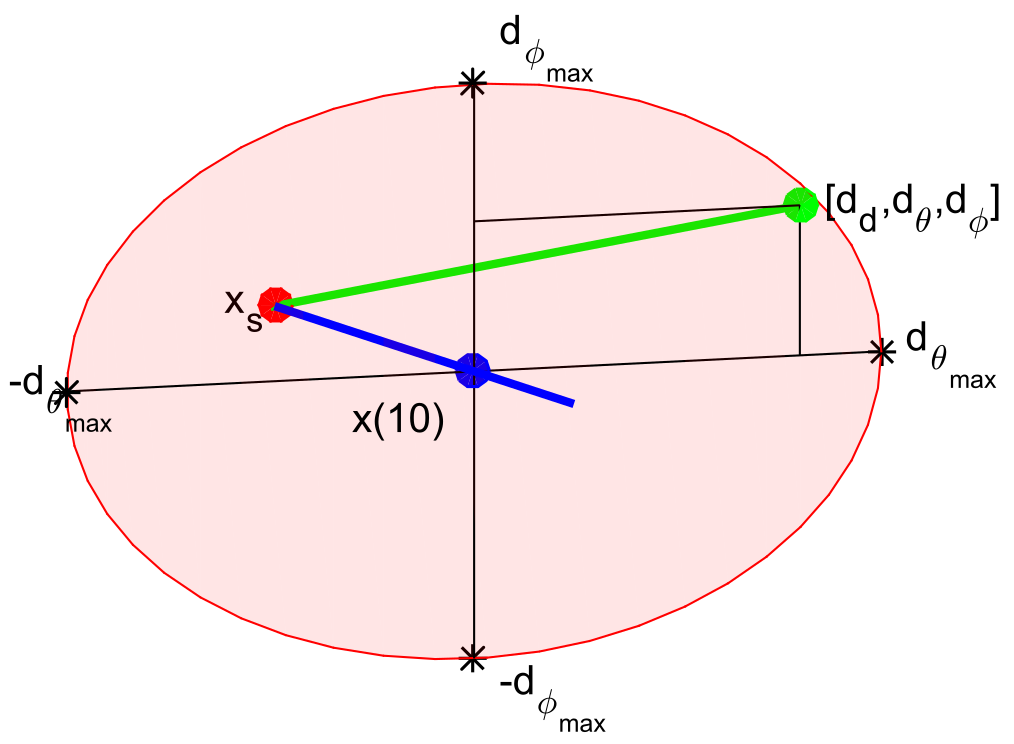
\includegraphics[width=0.7\textwidth]{\FIGDIR/TE014ElipticConeIOnePoint}         
    \caption{One rate position $[d_d,d_\theta,d_\varphi]$ (green). deviated from linear trajectory (blue line) at point ${x}(10)$.(blue) with initial position $x_s$ (red)}
    \label{fig:P21ElipticConeIOnePoint}
\end{figure}


The internal coordinate frame ${p}\in\R^2$ has origin in ${x}(t)\to\R^2$. The points of plane ${p}$ are bounded by projection ${p}=({b}-{x}(t))\to\R^2$, where $b\in D({x}(t),v)$. The point of ellipsoidal ${p}$ is then given as standard ellipse boundary with vertical span $d_\theta({x}(t))$ and horizontal span $d_\varphi({x}(t))$. 

The 2D \emph{Ellipsoid} $E({x}(t),{v})$ for specific time $t=10s$ example is portrayed  as red ellipsoid (in fig. \ref{fig:P21ElipticConeIOnePoint}).

\begin{equation}\label{eq:baseElipsoidxt}
    E({x}(t),{v})=\left\{ \begin{aligned}{b}\in\R^3:&{b}\in D({x}(t),{v}),{p}=({b}-{x}(t))\to\R^2,\\&\left(\frac{p(1)^2} {d_\theta({x}(t))^2}+ \frac{p(2)^2}{d_\varphi({x}(t))^2}\right)\le 1\end{aligned}\right\}
\end{equation}

\noindent The expected behavior of an intruder $i_k$ is to stick to predicted linear trajectory ${x}(t)$ (\ref{eq:vehiclelinearcone}). The probability of deviation should be decreasing with distance from the ellipse center (fig. \ref{fig:intruderPassingProbability}.).  


\noindent \emph{Probability density function} for ellipsoid  $E({x}(t),{v})$defined in (eq. \ref{eq:baseElipsoidxt}) is depending on maximal horizontal spread $d_\theta({x}(t))$, maximal vertical spread $d_\varphi({x}(t))$, defined by (eq. \ref{eq:elipsiodialBoudaryParameters}). 

Two standard probabilistic distributions are established $\mathscr{N}(\mu_\theta,\sigma_\theta)$ (eq. \ref{eq:elipsprobdistHorizontal}) for horizontal spread $\theta({x}(t))$ and $\mathscr{N}(\mu_\varphi,\sigma_\varphi)$  (eq. \ref{eq:elipsprobdistVertical}) for vertical spread $\varphi({x}(t))$. The means $\mu_\theta$ and $\mu_\varphi$ are set to zero, and internal coordinate frame ${p}\in\R^2$ where ${x}(t)\to\R^2$ is frame center. The variances $\sigma_\theta$ and $\sigma_\varphi$ are set as maximal distances on horizontal/vertical spread axes $d_\theta({x}(t))$ and $d_\varphi({x}(t))$.

\begin{equation}\label{eq:elipsprobdistHorizontal}
    P({x}(t),d_\theta)=\mathscr{N}(\mu_\theta,\sigma_\theta)=\mathscr{N}(0,d_\theta({x}(t)))
\end{equation}

\begin{equation}\label{eq:elipsprobdistVertical}
    P({x}(t),d_\varphi)=\mathscr{N}(\mu_\varphi,\sigma_\varphi)=\mathscr{N}(0,d_\varphi({x}(t)))
\end{equation}

\noindent The combined \emph{probability density function} for maximal spreads $d_\theta$ and $d_\varphi$ is given by (eq. \ref{eq:elipsprobdistCombined}). Because probability density function is defined for internal space ${p}\in\R^2$ and one may need to calculate impact rate for  cell space $c_{i,j,k}\in\R^3$. 

The reduction from two parameter probability distribution function to scalar rate distribution function is needed. A scalar rate distribution  function $P({x}(t),d_\theta,d_\varphi)$ over ellipsoid $E({x}(t),{v})$ is defined as (eq.\ref{eq:elipsprobdistCombined}), where the final rate is given as an average of two partial probabilities. 

Final space intersection rate $P({x}(t),d_\theta,d_\varphi)$ needs to be normalized to hold \emph{normal distribution condition} (eq. \ref{eq:normalDistrobitionCondition}). Normal distribution condition value (eq. \ref{eq:normalDistrobitionCondition}) is given as surface integral over ellipsoid $E({x}(0),{v})$ with rate distribution function $P({x}(t),d_\theta,d_\varphi)$.

\begin{equation}\label{eq:elipsprobdistCombined}
    P({x}(t),d_\theta,d_\varphi) = \frac{\mathscr{N}(\mu_\theta,\sigma_\theta)+\mathscr{N}(\mu_\varphi,\sigma_\varphi)}{2}
\end{equation}

\begin{equation}\label{eq:normalDistrobitionCondition}
    \iint_{E({x}(\tau))} P({x}(t),d_\theta,d_\varphi) \,\text{d}d_\theta\,\text{d}d_\varphi = 1
\end{equation}

\noindent Final space intersection rate  $P({x}(t),c_{i,j,k},\theta,\varphi)$  (space portion, time portion is calculated in (eq.\ref{eq:intruderIntersectionProbability}) is given by (eq. \ref{eq:spreadIntruderIntersectionProb}). Its mean value of all intersection rates $P({x}(\tau),c_{i,j,k},\theta,\varphi)$ where $\tau\in[i_e(c_{i,j,k}),i_l(c_{i,j,k})]$ is fixed point in intersection time interval.

An $P({x}(\tau),c_{i,j,k},\theta,\varphi)$ (\ref{eq:spreadIntersectionProbFixedtau}) is integration of rate density function $P({x}(\tau),d_\theta,d_\varphi)$ (eq. \ref{eq:elipsprobdistCombined}) in surface $E({x}(\tau),{v})$ to cell $c_{i,j,k}$ volume intersection. 

\begin{figure}[H]
    \centering
    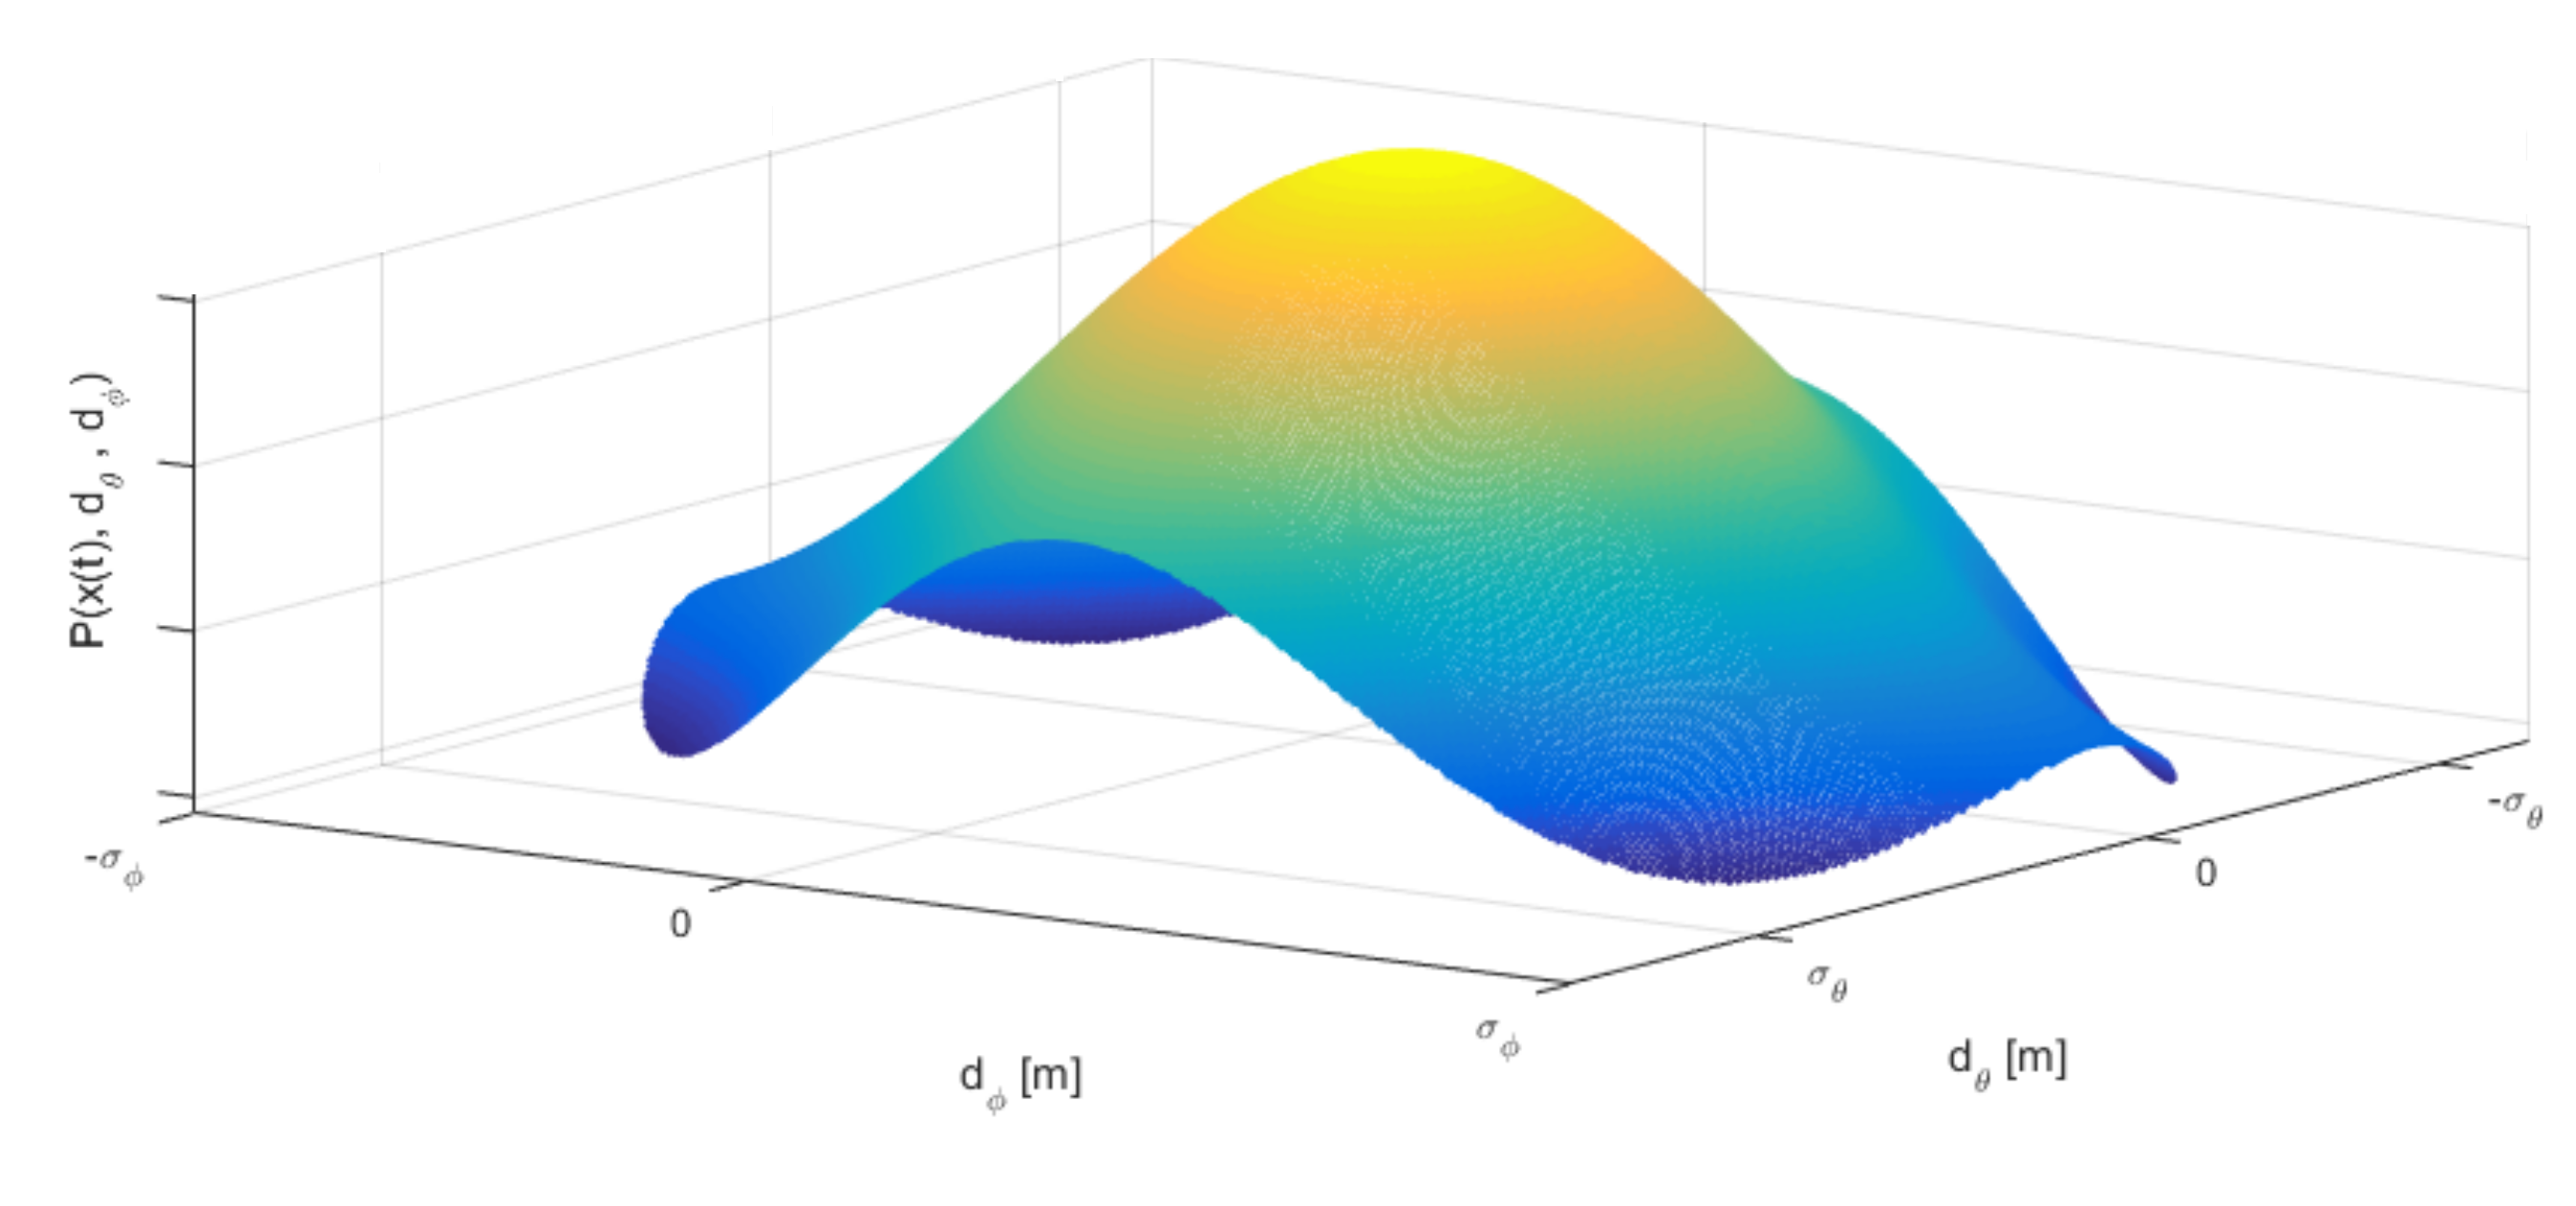
\includegraphics[width=0.9\textwidth]{\FIGDIR/TE015ProbabilisticDistributionOfEllipsoidCutSideForTE016}
    \caption{Probability of intruder $i_k$ position in ellipsoid $E({x}(t),{v})$}
    \label{fig:intruderPassingProbability}
\end{figure}

\noindent To get a volume integration partial rate in surface intersection must be integrated and normalized in time interval $\tau\in[i_e(c_{i,j,k}),i_l(c_{i,j,k})]$, the \emph{base intersection probability} $P_T(i_k({x}_s,{v},\theta,\varphi),c_{i,j,k})$ is given by (eq. \ref{eq:spreadIntruderIntersectionProb}). Example of intersection of intruder $i_r$ uncertain ellipsoid cone with avoidance grid $\mathscr{A}(t_i)$ is given in (fig. \ref{fig:ellipticConeIntersectionExample}).

\begin{equation}\label{eq:spreadIntersectionProbFixedtau}
    P({x}(\tau),c_{i,j,k},\theta,\varphi) =\iint_{E({x}(\tau),{v})\cap c_{i,j,k}} P({x}(\tau),d_\theta,d_\varphi)
\end{equation}

\begin{equation}\label{eq:spreadIntruderIntersectionProb}
    P_T(i_k({x}_s,{v},\theta,\varphi),c_{i,j,k})=\frac{\int_{i_e(c_{i,j,k})}^{i_l(c_{i,j,k})} P({x}(\tau),c_{i,j,k},\theta,\varphi)\,\text{d}\tau}{i_l(c_{i,j,k})-i_e(c_{i,j,k})}
\end{equation}

\begin{figure}[H]
    \centering
    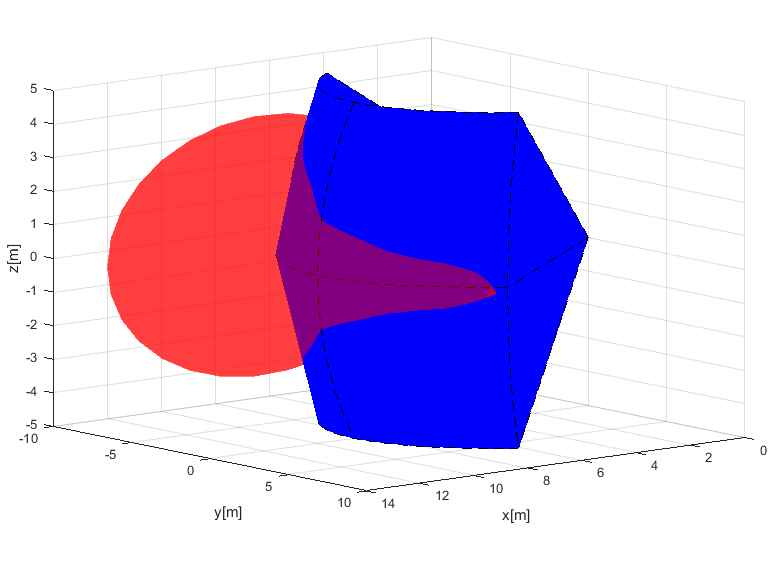
\includegraphics[width=0.7\textwidth]{\FIGDIR/TE013ElipticConeIntersecitonExample}
    \caption{Avoidance grid $\mathscr{A}(t_i)$ (blue) intersection with elliptic cone intruder $i_k({x},{v},\theta,\varphi)$ (red) example.}
    \label{fig:ellipticConeIntersectionExample}
\end{figure}

\noindent A \emph{numeric approximation} of space intersection rate $P_T(i_k({x}_s,{v},\theta,\varphi),c_{i,j,k})$ is more implementation feasible than symbolic calculation due to the multiple intersection constraints and bad intersection algorithm complexity. 

Let us define a homogeneous discrete subset of real numbers $\mathscr{R}$ which is a non-empty subset of real numbers $\R$. The set $\mathscr{R}$ (eq. \ref{eq:homogeneusdiscretizationofRealnumbers}) is homogeneous that means for an equal interval $(i,i+1],i\in\mathbb{Z}$ subset the count of members is equal to some positive natural number $k$. The parameter $k$ can be understood as \emph{unit approximation density}.

Similarly, the power sets $\mathscr{R}^2\subset\R^2$, $\mathscr{R}^3\subset\R^3$, ... $\mathscr{R}^i\subset\R^i,i\in\N^+$ keeps homogeneous distribution.

\begin{equation}\label{eq:homogeneusdiscretizationofRealnumbers}
    \mathscr{R} = \left\{\begin{aligned}a\in\R:&\forall i\in\mathbb{Z},|i<a\le i+1|=k,k\in\N^+, \\&\forall j\in \N^+a_{j+1}-a_{j}=m,m\in\R^+\end{aligned}\right\},\,\mathscr{R}\subset\mathbb{R}
\end{equation}

\noindent The orthogonal plane for ${x}(t), {v}, t \in\R$ is defined by (eq. \ref{eq:elisioidalOtrthogonalPlane}). The orthogonality property is also kept for any subspace $\mathscr{R}^n\in\R^n,n\in\N^+$. Numeric approximation of $D({x}(t),{v})$ is given as $D_D({x}(t),{v})$ (eq. \ref{eq:elisioidalOtrthogonalPlaneDiscrete}). 

The only difference is that discrete approximation is countable $|D_D|=m,m\in\N^+$, but continuous representation $|D|\approx \infty$ is uncountable. Because ellipsoid is a subset of orthogonal plane it keeps its countability property; therefore $E_D$ is also countable and must contain at least one member.

\begin{equation}\label{eq:elisioidalOtrthogonalPlaneDiscrete}
    D_D({x}(t),{v})=\left\{{a}\in\mathscr{R}^3:({a}-{x}(t))\perp{v},\right\},t\in\mathscr{R}
\end{equation}

\noindent The \emph{base ellipsoid} $E({x}(t),{v})$ for continuous-space is given by (eq. \ref{eq:baseElipsoidxt}). Every element, expect the base of internal projection $\mathscr{R}^2$ and orthogonal plane $D_D$ is same in discrete case $E_D({x}(t),{v})$ (eq. \ref{eq:baseElipsoidxtDiscrete}).

\begin{equation}\label{eq:baseElipsoidxtDiscrete}
    \bar{E}_D({x}(t),{v})=\left\{ \begin{aligned}{b}\in\mathscr{R}^3:&{b}\in D_D({x}(t),{v}),{p}=({b}-{x}(t))\to\mathscr{R}^2,\\&\left(\frac{p(1)^2} {d_\theta({x}(t))^2}+ \frac{p(2)^2}{d_\varphi({x}(t))^2}\right)\le 1\end{aligned}\right\},t\in\mathscr{R}
\end{equation}

\noindent The \emph{numeric calculation disproportion} can occur in case that ellipsoid $\bar{E}_D({x}(t),{v})$ (\ref{eq:baseElipsoidxtDiscrete}) in case of $d_\theta({x}(t))\approx 0$ and $d_\varphi({x}(t))\approx 0$. The count of ellipsoid members can be $|\bar{E}_D({x}(t),{v})|=0$, which is in contradiction with assumption $|\bar{E}_D({x}(t),{v})|\neq 0$. 

Let assume for discrete times $\tau=\left\{t_1,t_2,\dots,t_i\right\}$, $i\in \N^+$ there exists ellipsoids $\bar{E}_D({x}(t_1),{v})$,$\bar{E}_D({x}(t_1),{v})$, $\dots$, $\bar{E}_D({x}(t_i),{v})$ which are non empty and in space $\mathscr{R}^2$ in internal coordinate frame and space $\mathscr{R}^3$ in avoidance grid $\mathscr{A}(t_i)$ coordinate frame. The intersection of these partial ellipsoids in both spaces is equal to:

\begin{equation}
    \bar{E}_D({x}(t_1),{v})\cap \bar{E}_D({x}(t_2),{v})\dots\cap\dots \bar{E}_D({x}(t_i),{v}) = \varnothing
\end{equation}

\noindent An \emph{empty intersection} enables us to keep homogeneity property of ellipsoids by adding points so it is safe to add specific point ${x}(t)$ into empty ellipsoid. But only one, because it does not impact  probability density functions $\mathscr{N}(\mu_\theta,\sigma_\theta)$ and $\mathscr{N}(\mu_\varphi,\sigma_\varphi)$, neither space intersection rate  density function $P({x},d_\theta,d_\varphi)$. 

The final ellipsoid used forward $E_D({x}(t),{v})$(eq. \ref{eq:baseElipsoidxtDiscreteSafe}) is keeping all properties of ellipsoid $E({x}(t),{v})$ (eq. \ref{eq:baseElipsoidxtDiscreteSafe}). 

\begin{equation}\label{eq:baseElipsoidxtDiscreteSafe}
    E_D({x}(t),{v})= 
    \begin{cases}
        |\bar{E}_D({x}(t),{v})|=0 &: \left\{{x}(t)\right\} \\
        |\bar{E}_D({x}(t),{v})|\ge0 &: \bar{E}_D({x}(t),{v}) 
    \end{cases}
\end{equation}

\noindent The normal distribution condition for rate distribution function $P_D({x}(t),d_\theta,d_\varphi,{p})$, which is instance of to rate density function $P({x}(y),d_\theta,d_\varphi)$ (eq. \ref{eq:elipsprobdistCombined}) is used. This rate distribution must be normalized according to (eq.  \ref{eq:normalDistrobitionConditionDiscrete}).

\begin{equation}\label{eq:normalDistrobitionConditionDiscrete}
    \sum_{{p} \in E_D({x}(t))} P_D({x}(t),d_\theta,d_\varphi,{p}) = 1,\forall t\in\mathscr{R}^+
\end{equation}

\noindent The equations for \emph{space intersection rate} are similar to (eq. \ref{eq:spreadIntersectionProbFixedtau}, \ref{eq:spreadIntruderIntersectionProb}). For cell $c_{i,j,k}$ there exist intruder entry time $i_e(c_{i,j,k})$ its the earliest intersection with ellipsoid $E_D({x}(i_e(c_{i,j,k}))),{v}$. Same situation occurs with intruder leave time $i_l(c_i,j,k)$. Because $E_D$ is countable set, it means additional attributes can be attached to each point ${p}\in E_D$. Based on system dynamic (eq. \ref{eq:intruderBasicLinearModel}) the \emph{Time Of Arrival} (TOA) can be calculated. The example of TOA is given in fig. \ref{fig:intruderTimeOfArrival}.

\begin{figure}[H]
    \centering
    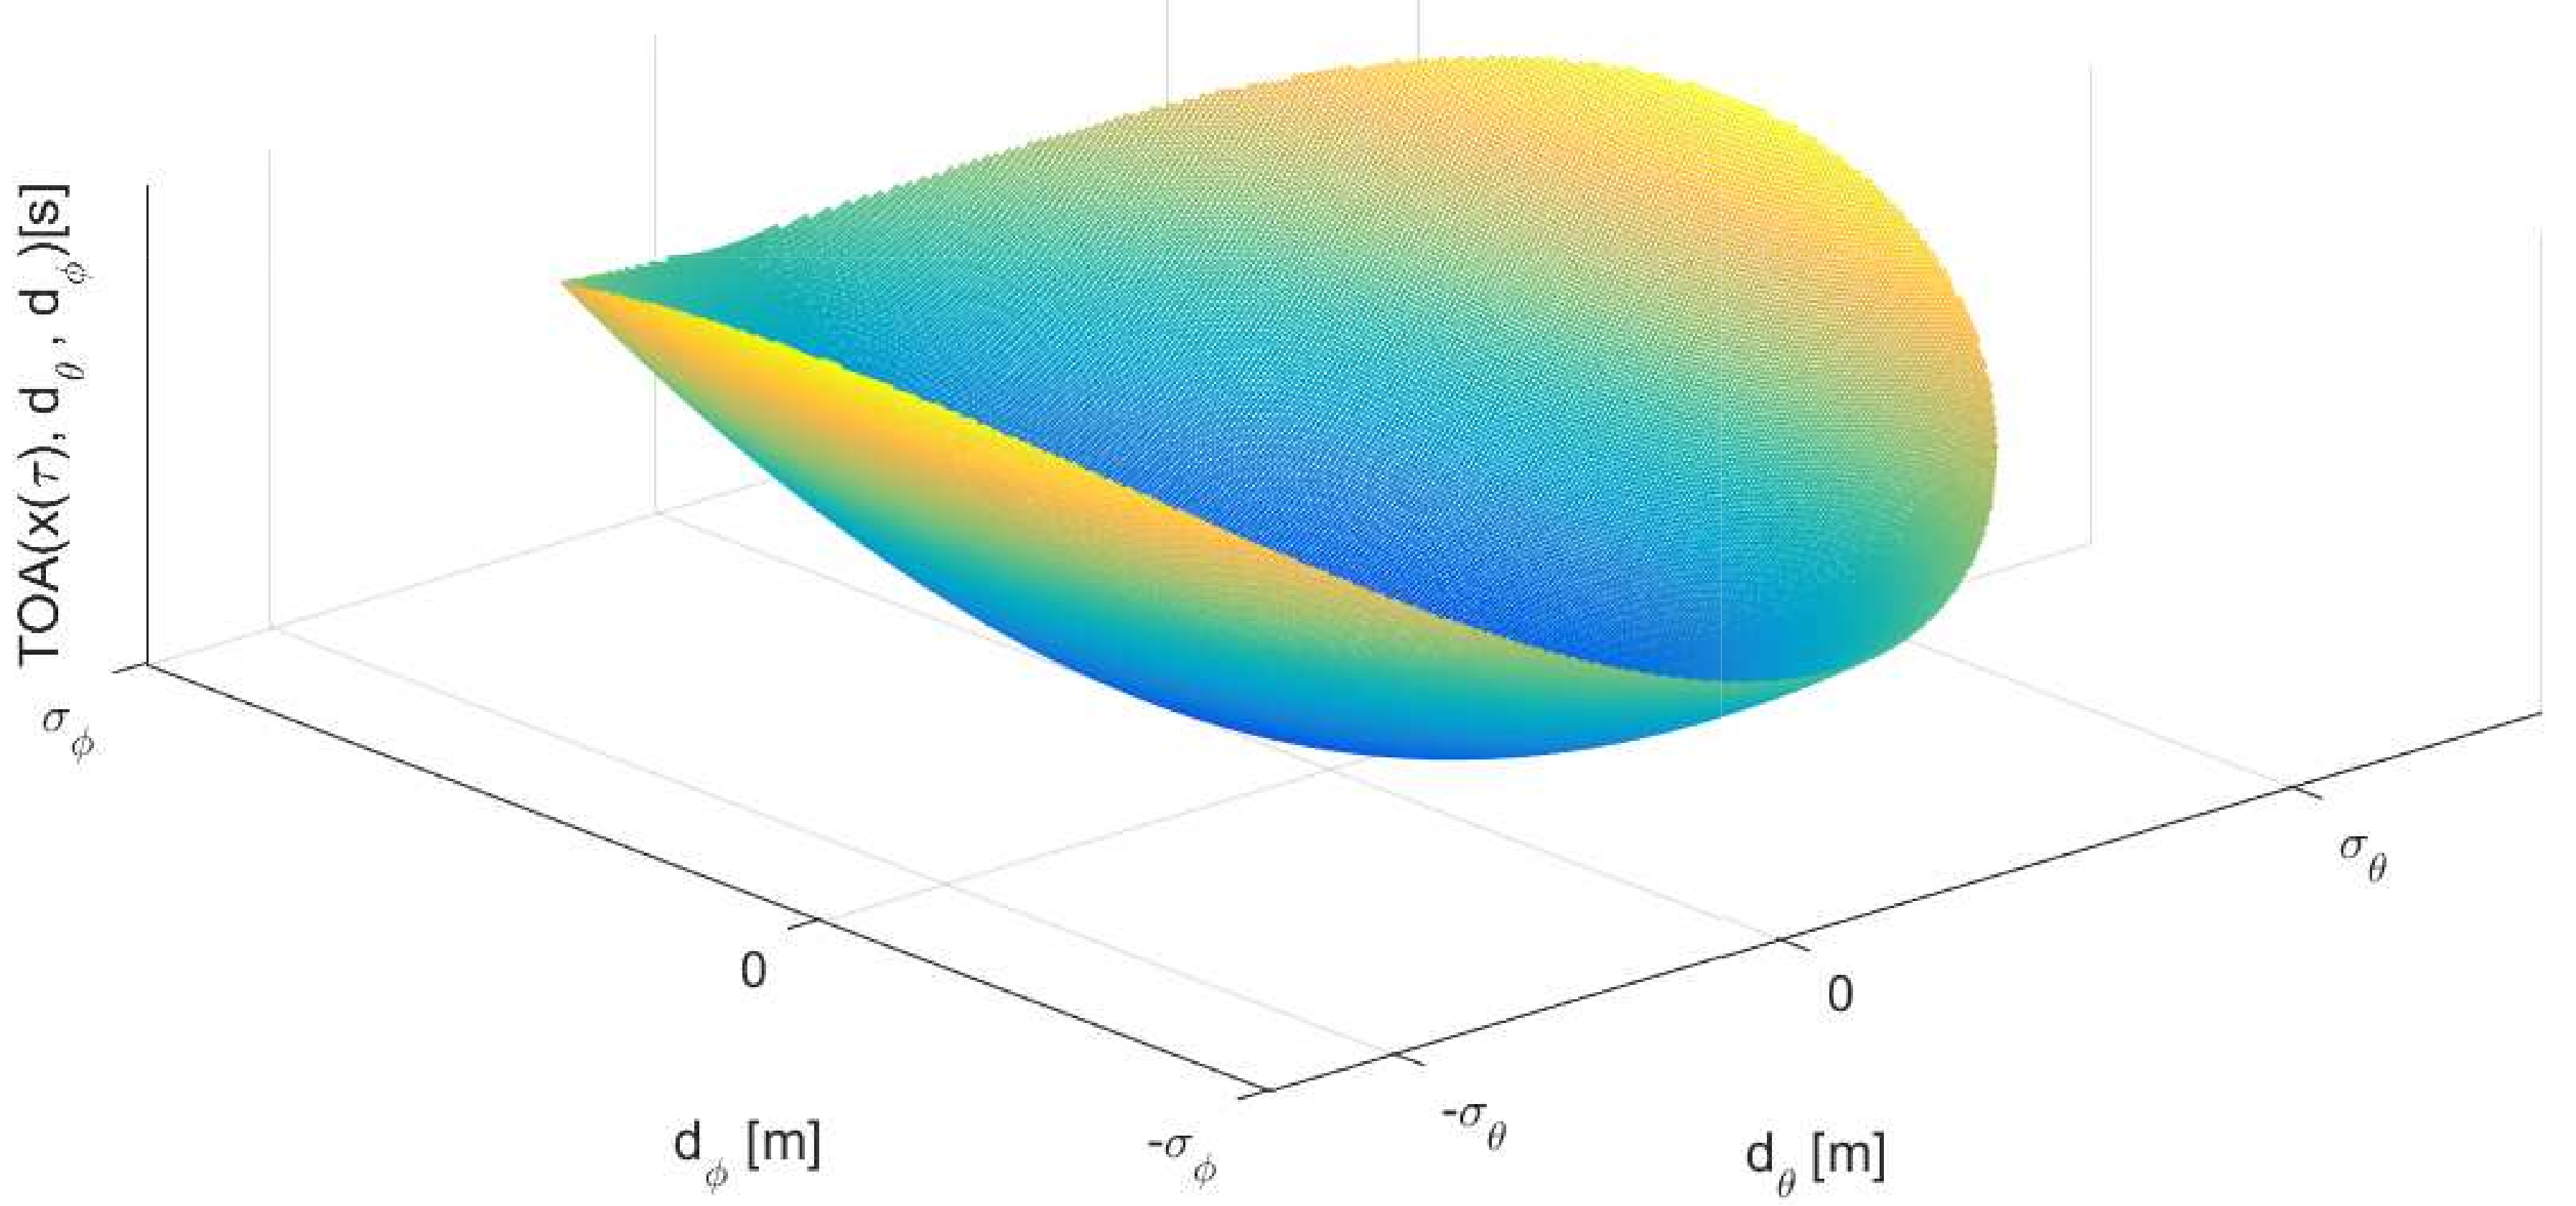
\includegraphics[width=0.7\textwidth]{\FIGDIR/TE016EllipsoidCutTimeOfArrival} 
    \caption{Time Of Arrival (TOA) for one ellipsoid $E_D({x}(\tau),{v})$.}
    \label{fig:intruderTimeOfArrival}
\end{figure}

\noindent The intersection rate $P_D({x}(\tau),c_{i,j,k},\theta,\varphi)$ for one time sample $\tau$ is given by (eq. \ref{eq:spreadIntersectionProbFixedtauDiscrete}), which has similar notation to (eq. \ref{eq:spreadIntersectionProbFixedtau}), sums are used instead of integrals and discrete rate density function $P_D({x}(\tau),d_\theta,d_\varphi,{p})$ for points form ellipse and cell intersection are used as iterator base set ${p}\in\left\{E_D({x}(\tau),{v})\cap c_{i,j,k}\right\}$.

\begin{equation}\label{eq:spreadIntersectionProbFixedtauDiscrete}
    P_D({x}(\tau),c_{i,j,k},\theta,\varphi) =\sum_{{p}\in \left\{E_D({x}(\tau),{v})\cap c_{i,j,k}\right\}} P_D({x}(\tau),d_\theta,d_\varphi,{p})
\end{equation}

\noindent The \emph{space intersection rate} $P_{TD}(i_k({x}_s,{v},\theta,\varphi),c_{i,j,k})$ (eq. \ref{eq:spreadIntruderIntersectionProbDiscrete}) is given as mean intersection rate of partial intersections $P_D({x}(\tau),c_{i,j,k},\theta,\varphi)$ where step set $T=\{$ $i_e(c_{i,j,k})$, $\dots$, $i_l(c_{i,j,k})\}$ contains all viable intersection times with ellipsoids $E({x}(\tau\in T),{v})$. The denominator is basically count of samples in sample time set $T$. 

\begin{equation}\label{eq:spreadIntruderIntersectionProbDiscrete} 
    P_{TD}(i_k({x}_s,{v},\theta,\varphi),c_{i,j,k})=\frac{\sum_{\tau=i_e(c_{i,j,k})}^{i_l(c_{i,j,k})} \sum_{{p}\in E_D({x}(\tau),{v})}P_D({x}(\tau),c_{i,j,k},\theta,\varphi,{p})}{\sum_{\tau i_l(c_{i,j,k})}^{i_e(c_{i,j,k})} 1}
\end{equation}

\noindent An \emph{intersection of intruder cone and cell} $c_{i,j,k}$ cell is defined by (eq. \ref{eq:conicIntersectionCellIntruderDiscrete}) The  set of point ${p}\in\mathscr{R}^3$ where condition of intersection between ellipsoids $E_D({x}(\tau),{v})$ for times $\tau\in\mathscr{R}^+$ and cell space $c_{i,j,k}$ is met.

\begin{equation}\label{eq:conicIntersectionCellIntruderDiscrete}
    \mathscr{P}(i_k({x}_s,{v},\theta,\varphi),c_{i,j,k})= \bigcup_{\forall \tau\in\mathscr{R}^+} \left\{{p}\in\mathscr{R}^3:{p}\in c_{i,j,k}\cap E_D({x}(\tau),{v})\right\}
\end{equation}

\noindent An \emph{intruder time of entry} $i_e(i_k,c_{i,j,k})$ (eq. \ref{eq:conicTimeOfEntryDiscrete}), for intruder $i,k$ and cell $c_{i,j,k}$ is approximated for discrete point set  $\mathscr{P}(i_k({x}_s,{v},\theta,\varphi),c_{i,j,k})$ (eq. \ref{eq:conicIntersectionCellIntruderDiscrete}) as minimal time of arrival $t_{TOA}({p})$ of member points ${p}$.

\begin{equation}\label{eq:conicTimeOfEntryDiscrete}
    i_e(i_k,c_{i,j,k})\approx \min \left\{t_{TOA}({p}):{p}\in\mathscr{P}(i_k({x}_s,{v},\theta,\varphi),c_{i,j,k})\right\}
\end{equation}

\noindent An \emph{intruder time of leave} $i_l(i_k,c_{i,j,k})$ (eq. \ref{eq:conicTimeOfLeaveDiscrete}), for intruder $i,k$ and cell $c_{i,j,k}$ is approximated for discrete point set  $\mathscr{P}(i_k({x}_s,{v},\theta,\varphi),c_{i,j,k})$ (eq. \ref{eq:conicIntersectionCellIntruderDiscrete}) as maximal time of arrival $t_{TOA}({p})$ of member points ${p}$.

\begin{equation}\label{eq:conicTimeOfLeaveDiscrete}
    i_l(i_k,c_{i,j,k})\approx \max \left\{t_{TOA}({p}):{p}\in\mathscr{P}(i_k({x}_s,{v},\theta,\varphi),c_{i,j,k})\right\}
\end{equation}

\paragraph{Combined intersection model:} The \emph{combined intersection model} $P_{O_I}(i_k,c_{i,j,k},l,b,s,\tau)$ is defined for intruder $i_k$ with parameters:

\begin{enumerate}
    \item\textit{Starting position} ${x}_s$ - expected position of intruder $i_r$ in 3D space at time of avoidance $t_i$ in avoidance grid frame $\mathscr{A}(t_i)$.
    
    \item\textit{Velocity vector} ${v}$ - oriented velocity of intruder $i_r$ at time of avoidance $t_i$ in avoidance grid frame $\mathscr{A}(t_i)$. 
    
    \item\textit{Horizontal uncertainty spread} $\theta$ - defines how much can intruder $i_r$ deviate on horizontal axis of intruder local coordinate frame (if X+ is the main axis, then Y is horizontal axis in right-hand euclidean coordinate frame), due the properties of intersection definition, the horizontal uncertainty spread can have following values $\theta\in[0,\pi/2]$.
    
    \item\textit{Vertical uncertainty spread} $\varphi$ -defines how much can intruder $i_r$ deviate on vertical axis of intruder local coordinate frame (if X+ is the main axis in local right-hand euclidean intruder coordinate frame, then Z is horizontal-vertical axis), due to the intersection definition, the vertical uncertainty spread can have following values $\varphi\in[0,\pi/2]$.
    
    \item\textit{Body volume radius} $r$ - defines the body volume of an intruder in meters and it has  $\R^+$  value.
\end{enumerate}

\noindent The \emph{flag vector} $l,b,s,\tau \in \left\{0,1\right\}$ is a parametrization  of rate calculation: $l$ stands for the \emph{lined intersection}, $b$ stands for \emph{body intersection}, $s$ stands for the \emph{spread intersection}, $\tau$ stands for \emph{time account}. 

The \emph{space intersection for line} $P_L(i_k,c_{i,j,k})$ is defined as $P_T(i_k({x},{v}),c_{i,j,k})$, where $i_k$ is intruder with properties of initial position ${x}$, velocity vector ${v}$ and $c_{i,j,k}$ is target cell. (eq. \ref{eq:baseIntersectionProbabilityLineIntersectionType}). 

The \emph{space intersection rate for body volume} $P_B(i_k,c_{i,j,k})$ is defined as $P_T(i_k({x},{v},r),c_{i,j,k})$ (eq. \ref{eq:baseIntersectionProbabilityBallIntersectionType}), where intruder $i_r$ has additional property of the intruder body volume radius $r$. 

The \emph{space intersection probability for maneuverability uncertainty} $P_S(i_k,c_{i,j,k})$ is defined as $P_{TD}(i_k({x}_s,{v},\theta,\varphi),c_{i,j,k})$ (eq. \ref{eq:spreadIntruderIntersectionProbDiscrete}), where intruder properties $\theta$, $\varphi$ stands for intruder horizontal and vertical uncertainty spread.

The \emph{time intersection rate} $P_{\tau,x}(i_k,c_{i,j,k})\in[0,1]$ is defined in (eq. \ref{eq:intruderIntersectionProbability}). This probability has two calculation modes, first is for 1D intersection (line), second is for volume intersection (body volume, spread elliptic cone).  

UAS cell entry time $t_e$ and cell leave time  $t_l$ time for a vehicle in avoidance grid $\mathscr{A}(t_i)$ is given by (eq. \ref{eq:cellEntryTime}) and (eq. \ref{eq:cellLeaveTime}). 

Intruder leave and entry time for 1D intersections is trivial and is omitted in this section. Intruder entry $i_e$ and intruder leave $i_l$ for 3D intersection is given by (eq. \ref{eq:conicTimeOfEntryDiscrete}, \ref{eq:conicTimeOfLeaveDiscrete}). 

All partial rates with respective definition references are summarized in (eq. \ref{eq:partialProbabilitiesIntruderSummary})

\begin{equation}\label{eq:partialProbabilitiesIntruderSummary}
    \begin{aligned}
        P_L(i_k,c_{i,j,k}) &= P_T(i_k({x},{v}),c_{i,j,k}) &(\ref{eq:baseIntersectionProbabilityLineIntersectionType})\\
        P_B(i_k,c_{i,j,k}) &= P_T(i_k({x},{v},r),c_{i,j,k}) &(\ref{eq:baseIntersectionProbabilityBallIntersectionType})\\
        P_S(i_k,c_{i,j,k}) &= P_{TD}(i_k({x}_s,{v},\theta,\varphi),c_{i,j,k}) &(\ref{eq:spreadIntruderIntersectionProbDiscrete})\\
        P_{\tau,x}(i_k,c_{i,j,k})&=\frac{\norm{[i_e(c_{i,j,k}),i_l(c_{i,j,k})]\cap [t_e,t_l]}}{\norm{[t_e,t_l]}}& (\ref{eq:intruderIntersectionProbability})\\
    \end{aligned}
\end{equation}

\noindent With definition of all space and time intersection rates (eq. \ref{eq:partialProbabilitiesIntruderSummary}) and given flag vector $l,b,s,\tau \in\left\{0,1\right\}$ one can formulate combined intersection rate $P_{O_I}(i_k,c_{i,j,k},l,b,s,\tau)$ (eq. \ref{eq:intruderInCellProbabilityOneIntruder}) for intruder $i_k$ and cell $c_{i,j,k}$. The principle is following: \emph{maximum of selected rates product based on flag vector is final intersection rate of intruder $i_k$ in the cell}. 

The time-use flag $\tau$ is adding time intersection rate $P_{\tau,x}(i_k,c_{i,j,k})$, where time intersection rate is defined by $x=\left\{L,B,S\right\}$ for line, body volume, spread ellipse time intersections ($P_{\tau,L}(i_k,c_{i,j,k})$ $\neq$ $P_{\tau,B}(i_k,c_{i,j,k})$ $\neq$ $P_{\tau,B}(i_k,c_{i,j,k})$ for one intruder $i_k$).

\begin{equation}\label{eq:intruderInCellProbabilityOneIntruder}
    \begin{aligned}
        P_{O_I}(i_k,c_{i,j,k},l,b,s,\tau) & = \begin{cases}\tau=0&:\max\left\{\begin{aligned}P_L(i_k,c_{i,j,k}).l\\ P_B(i_k,c_{i,j,k}).b\\P_S(i_k,c_{i,j,k}).s\end{aligned}\right\}\\\tau=1&:\max\left\{\begin{aligned}P_{\tau,L}(i_k,c_{i,j,k}).P_L(i_k,c_{i,j,k}).l\\ P_{\tau,B}(i_k,c_{i,j,k}).P_B(i_k,c_{i,j,k}).b\\P_{\tau,S}(i_k,c_{i,j,k}).P_S(i_k,c_{i,j,k}).s\end{aligned}\right\}\end{cases} &\\
    \end{aligned}
\end{equation}
    	\subsection{(W) Moving Constraints}\label{s:MovingVirtualConstraints}
\paragraph{Idea:} The basic ideas is the same as in case \emph{static constraints} (sec. \ref{s:virtualConstraints}). There is horizontal constraint and altitude constraint outlining the constrained space. The only additional concept is moving of \emph{constraint} on horizontal plane in global coordinate system. 

The constraint intersection  with \emph{avoidance grid} is done in \emph{fixed decision Time}, for cell in \emph{fixed cell leave time} (eq. \ref{eq:cellLeaveTime}), which means concept from static obstacles can be fully reused.

\paragraph{Definition:} The \emph{moving constraint definition} (eq. \ref{eq:movingConstraintDefinition}) covers minimal data scope for  moving constraint, assuming linear constraint movement. 

The original definition (eq. \ref{eq:staticConstraint}) is enhanced with additional parameters to support constraint moving:

\begin{enumerate}
    \item \emph{Velocity} - velocity vector on 2D horizontal plane.
    
    \item \emph{Detection time} - the time when \emph{constraint} was created/detected, this is the time when \emph center and boundary points position were valid.
\end{enumerate}

\begin{multline}\label{eq:movingConstraintDefinition}
    constraint = \{position,boundary,\dots\\\dots, velocity, detection Time, \dots \\\dots altitude_{start},altitude_{end}, safety Margin\}
\end{multline}

\paragraph{Cell Intersection:} The \emph{intersection algorithm} follows (eq. \ref{eq:contraintToCellIntersection}), only shift of the \emph{center and boundary points} is required. 

First let us introduce $\Delta time$ (eq. \ref{eq:deltatimeMovingconst}), which represents difference between the constraint detection time and expected cell leave time (eq. \ref{eq:cellLeaveTime}).

\begin{equation}\label{eq:deltatimeMovingconst}
    \Delta time = UAS_{leave}(cell_{i,j,k}) - detection Time
\end{equation}

\noindent The constraint boundary is shifted to:

\begin{multline}
    shifted Boundary(constraint) = \{new Point = point + velocity \times \Delta time:\dots\\\dots \forall point \in constraint.boundary \}
\end{multline}

\noindent The constraint center is shifted to:

\begin{equation}
    shifted Center(constraint) = constraint.center + velocity
\end{equation}

\begin{note}
    The $\Delta time$ is calculated separately for each $cell_{i,j,k}$, because \emph{UAS} is also  moving and reaching cells in different times. The \emph{cell leave time} can be calculated in advance after reach set approximation.
\end{note}

\paragraph{Alternative Intersection Implementation:} The alternative used for intersection selected based on polygon intersection algorithms review \citep{bentley1979algorithms}, the selected algorithm  is \emph{Shamos-Hoey} \cite{shamos1976geometric}.

The implementation was tested on \emph{Storm scenario} (sec. \ref{s:testStorm}) and it yelds same results.

   
    

%09-Bibliography
    \bibliography{thesis}
\end{document}
